\chapter{Other Elements}

This section shows you how to add other elements, like figurs or tables, to your document.

\section{Tables}

\subsection{Simple}

\begin{center}
\begin{tabular}{lrr}
	\toprule
	Description & Count & Price (single)\\
	\midrule
	Soda & 6 & 2.49 €\\
	Coffee & 2 & 3.19 €\\
	Sandwich & 1 & 5.39 €\\
	\bottomrule
\end{tabular}
\end{center}

\subsection{Specific Width}

\begin{center}
\begin{tabularx}{0.75\textwidth}{Xrr}
	\toprule
	Description & Count & Price (single)\\
	\midrule
	Soda & 6 & 2.49 €\\
	Coffee & 2 & 3.19 €\\
	Sandwich & 1 & 5.39 €\\
	\bottomrule
\end{tabularx}
\end{center}

\subsection{With Caption}

\Cref{tbl:some_table} as a caption and can be referenced.
Note that by using the \texttt{table} environment, the table is no longer inline and is repositioned automatically.

\begin{table}
	\centering
	\begin{tabularx}{0.75\textwidth}{Xrr}
		\toprule
		Description & Count & Price (single)\\
		\midrule
		Soda & 6 & 2.49 €\\
		Coffee & 2 & 3.19 €\\
		Sandwich & 1 & 5.39 €\\
		\bottomrule
	\end{tabularx}
	\caption{This table has a caption.}
	\label{tbl:some_table}
\end{table}

\section{Graphics}

Avoid having inline figures.
Always give them a caption and reference them in text.

\subsection{Figures}

See \cref{fig:some_figure}.

\begin{figure}
	\centering
	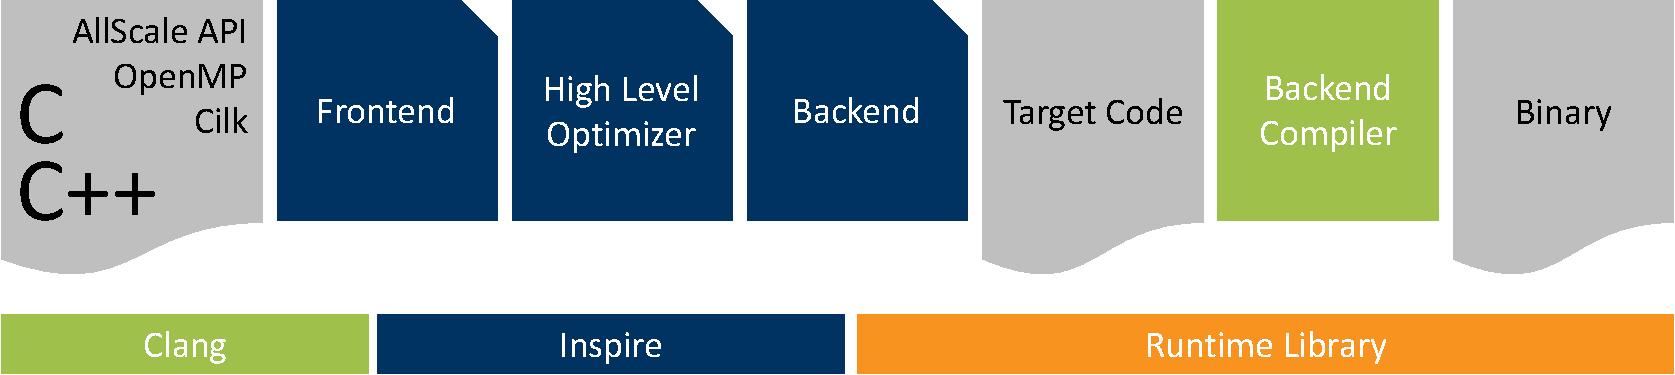
\includegraphics[width=0.9\textwidth]{images/example.pdf}
	\caption{An example image.}
	\label{fig:some_figure}
\end{figure}

\subsection{TikZ}

See \cref{fig:tikz_figure}.

\begin{figure}
	\centering
	%\usetikzlibrary{arrows.meta}
%\usetikzlibrary{positioning}

\tikzstyle{ptr} = [
	-{Latex[length=1.8mm]},
	dashed,
	shorten <= 0.2cm,
	shorten >= 0.2cm,
	bend left
]

\begin{tikzpicture}[every node/.style={minimum width=1cm},
                    level 1/.style={sibling distance=4.5cm},
                    level 2/.style={sibling distance=2.0cm}]

	\node (1) {\{\}}
		child {
			node (2) {$=$}
			child { node (3) {$a$} }
			child { node (4) {$6$} }
		}
		child {
			node (5) {$=$}
			child { node (6) {$b$} }
			child { node (7) {$7$} }
		}
		child {
			node (8) {call}
			child { node (9)  {$b$} }
			child { node (10) {$a$} }
			child { node (11) {$f$} }
		}
	;

	\foreach \n in {1,...,11} {
		\fill [black,opacity=.5] (\n.west) circle (1.5pt);
		\fill [black,opacity=.5] (\n.east) circle (1.5pt);
	}

	\path[ptr] (2.west)  edge                (1.west)
	           (3.west)  edge                (2.west)
	           (3.east)  edge                (3.west)
	           (4.west)  edge                (3.east)
	           (4.east)  edge                (4.west)
	           (2.east)  edge                (4.east)
	           (5.west)  edge[bend right=15] (2.east)
	           (6.west)  edge                (5.west)
	           (6.east)  edge                (6.west)
	           (7.west)  edge                (6.east)
	           (7.east)  edge                (7.west)
	           (5.east)  edge                (7.east)
	           (8.west)  edge[bend right=15] (5.east)
	           (9.west)  edge                (8.west)
	           (9.east)  edge                (9.west)
	           (10.west) edge                (9.east)
	           (10.east) edge                (10.west)
	           (11.west) edge                (10.east)
	           (11.east) edge                (11.west)
	           (8.east)  edge                (11.east)
	           (1.east)  edge                (8.east)
	;

\end{tikzpicture}

	\caption{An example figure using TikZ.}
	\label{fig:tikz_figure}
\end{figure}

\section{Source Code}

\subsection{Inline Code}

\begin{lstlisting}[language=c]
#include <stdio.h>
#include <stdlib.h>

int main(void)
{
	puts("Hello World\n");
	return EXIT_SUCCESS;
}
\end{lstlisting}

\subsection{External File}

\lstinputlisting[language=c]{code/sample.c}

\subsection{Listing}

See \cref{lst:some_listing}.

\lstinputlisting[language=c,float,caption={Some source code.},label={lst:some_listing}]{code/sample.c}

\subsection{Minted}

Minted is an external tool that provides syntax highlighting for various different languages.
See \cref{lst:minted_example} for an example.
Consider using it instead of the regular \texttt{listings} package.
Mixing them is not recommended as they do not look exactly the same.
Code can be written inline and taken from external files.

\begin{listing}
	\inputminted{haskell}{code/sample.hs}
	\caption{Example source code, using the \texttt{minted} package.}
	\label{lst:minted_example}
\end{listing}
